Les résultats précédents montrent qu'il reste encore quelques cas d'échecs de convergence pour les réseaux $\mathcal{S}$MorphNetTanh à deux couches morphologiques, avec les opérations cibles d'ouverture et de fermeture, et ce malgré l'ajout d'un partage doux des poids entre les noyaux $w$ des deux couches et l'ajout dans la \textit{loss} d'une contrainte $C_\text{awayOPP}$ entre les deux paramètres de contrôle $\alpha$ (ou $p$) associés. \\

\vspace{-1.4mm}
\noindent La modulation de l'initialisation des noyaux $w$ du réseau devient alors une solution potentielle à ces derniers échecs. ALors que les poids des noyaux sont originellement initialisés selon une loi normale centrée réduite afin de brasser les différents états de convergence possibles à partir d'initialisations aléatoires différentes sur plusieurs expériences, on peut finalement se dire que cette forme initiale des noyaux peut être fixée et définie de manière déterminée au préalable, selon des caractéristiques morphologiques générales à priori que l'on connait ou que l'on recherche sur ces noyaux. \\

\vspace{-1.4mm}
\noindent En l'occurence, on peut facilement s'imaginer que ce que l'on recherche ou favorise dans nos différents cas d'étude, c'est une forme de noyaux centrée sur son support et peu dispersée. On choisira alors une initialisation sous la forme d'une gaussienne 2D, allant de $0$ aux coins de l'image des noyaux à $1$ en son centre (voir figure \ref{fig:init_gauss} suivante). \\


%figure
\vspace{-1.0mm}
\begin{figure}[htp]
  \begin{center}
    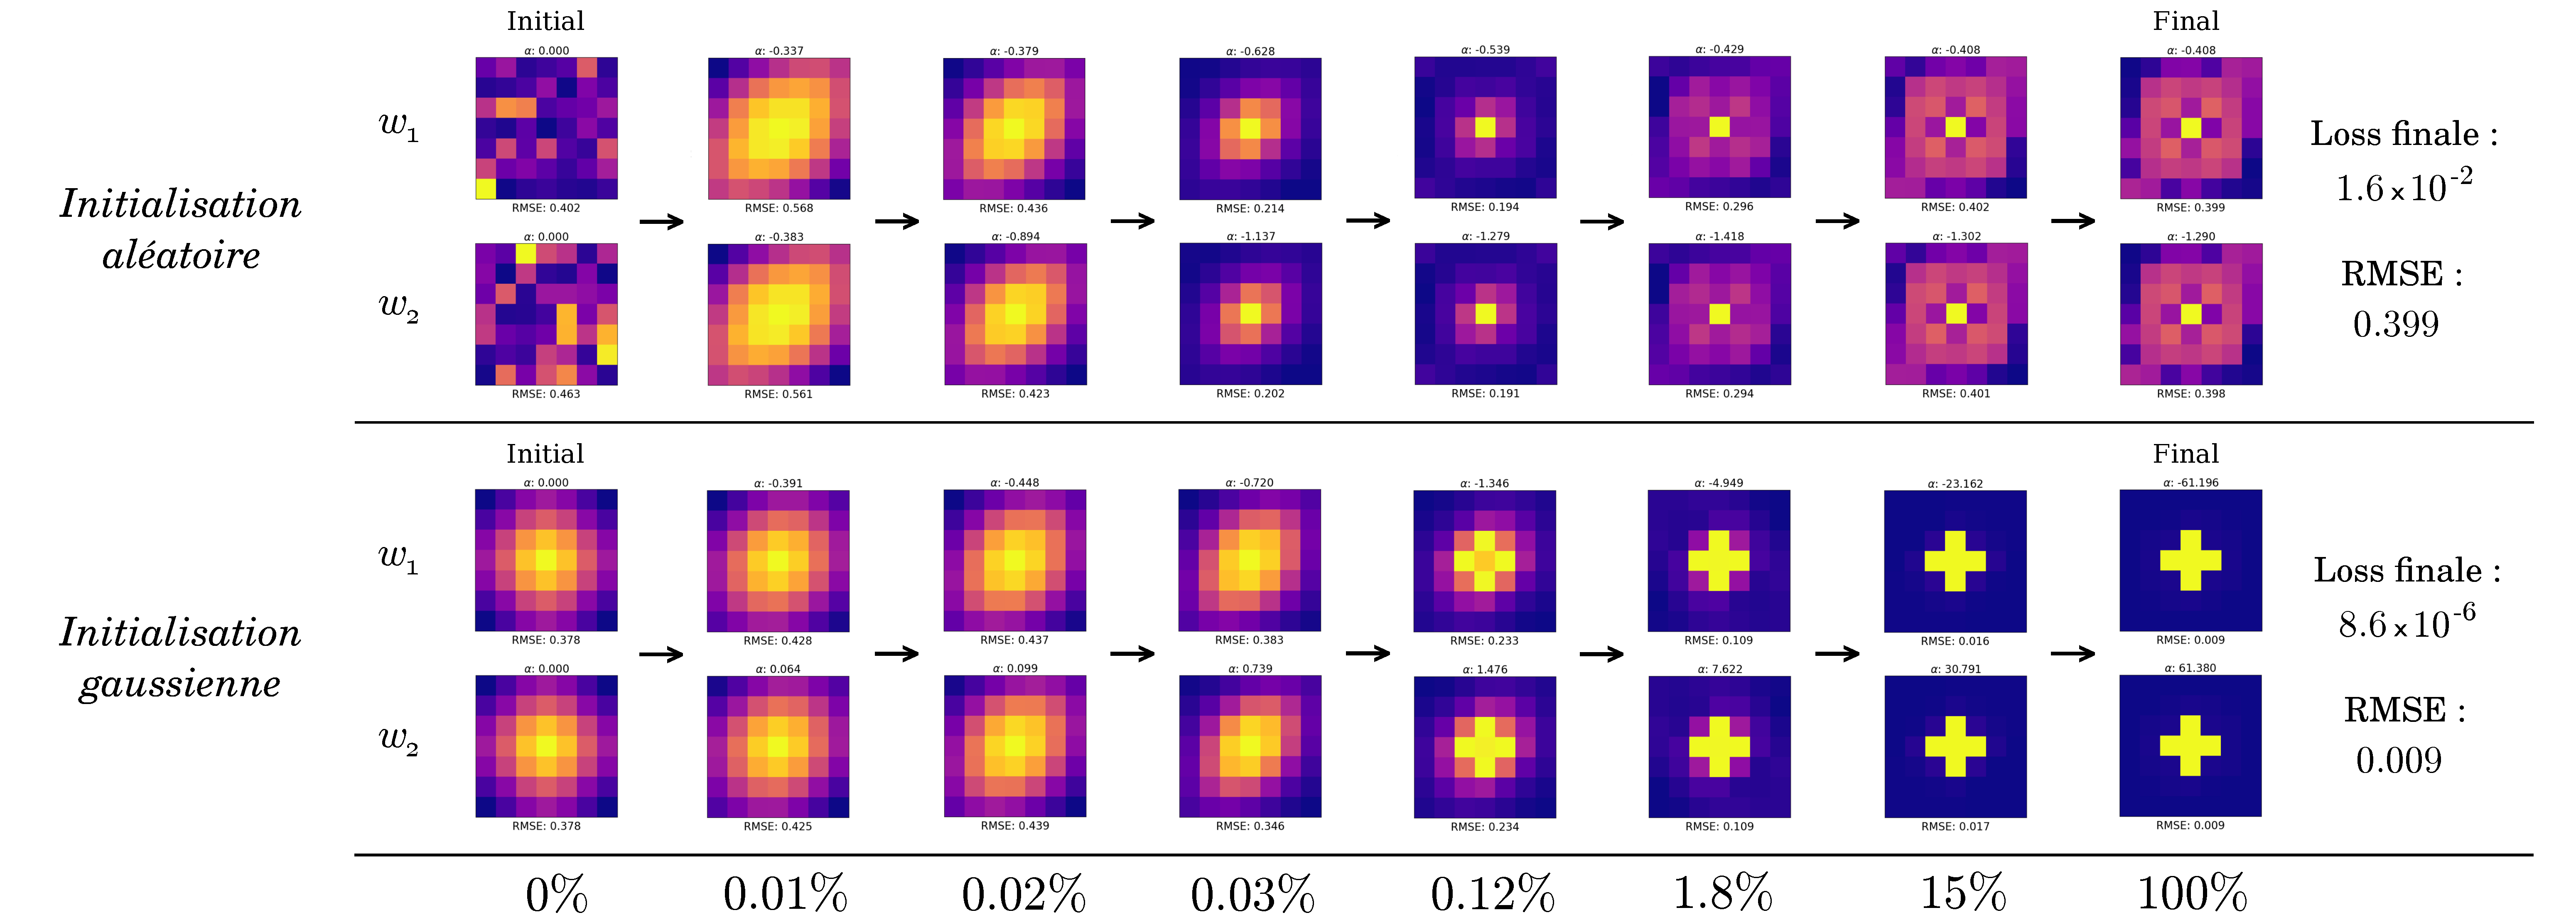
\includegraphics[width=1.00\linewidth]{parts/3-contributions/D-modulation_de_l_initialisation/figures/k_gauss.pdf}
    \vspace{-4.0mm}
    \caption{ \centering Évolution de la forme du noyau des deux couches du réseau et de sa \textit{RMSE} en fonction de la progression de l'entraînement (en \% avant l'état final), pour le \textit{cross3} et l'ouverture sur la banque MNIST, avec initialisation aléatoire et init. gaussienne.}
    \label{fig:init_gauss}
  \end{center}
\end{figure}


\vspace{-3.0mm}
\noindent L'exemple fig. \ref{fig:init_gauss}, obtenu sur six runs, montre bien ici l'efficacité de cette initialisation gaussienne des noyaux $w$ par rapport à l'aléatoire normale centrée réduite sur \textit{cross3} pour l'ouverture sur MNIST, avec des valeurs de \textit{RMSE} et de \textit{loss} bien plus faibles.
